% Paper on fault injection mechanisms: Authors Thorsten Piper et.al

\section{On the effective use of Fault injection for the assessment of AUTOSAR safety mechanism} % Major section
%------------------------------------------------
\subsection{Key Idea} % Sub-section
AUTOSAR safety standard ISO26262 strongly recommends usage of the fault injection standards, but no definite mechanism exists for enforcing the same.
Representation of the faults using the standard fault models e.g. bit flips and data type based corruption are not sufficient to model real time behavior.
The existing Fault Injection framework GRINDER is extended to support AUTOSAR and an assessment is provided.
%-----------------------------------------------
\subsection{Width and scope} % Sub-section
Provide open source and ready to use framework to do Fault Injection. Dependability  assessment on existing AUTOSAR timing monitor safety mechanism for identifying 
deficiencies and guidelines for derivation of special fault models, injection mechanisms and locations based on abstract AUTOSAR and ISO26262 fault models.
Eariler approach mentioned include: Lanigan et.al. and Baugarten et al. First approach being based on VECTOR CaNoe and second approach used anotated SWC Component to 
introduce fault ports. Another approach is pre implementation testing using UML or AADL, in this failure level are assumed and the effect on model analysed.
Vedder et. al extended property based testing to AUTOSAR. Here automated test cases were generated from a pre specified property files.

Hardware based FI: Modeling hardware error such as CAN bus failure, or NVRAM failure through corrupted CRC. Hardware based FI fails to handle component interaction and
dependability property.
Software based FI: e.g. BeSafe framework to intercept SWC calls and fuzzing error models to check resilience of SWC. GOOFI-2 to evaluate bit flip cases and  MODIFI to check model
at Simulink level.\\
\textbf{Note:} Simultaneous fault models with multiple points of failure completely missing from AUTOSAR standards.

%------------------------------------------------

\subsection{Experimental approach} % Sub-sub-section
\textbf{Configuration}: Target is instrumented with injectors and detectors,.
\textbf{Execution:} The target system is executed till the injection of fault and the perturbation data is successfully completed.
\textbf{Evaluation:} The logs and traces are collected.
GRINDER extended to AUTOSAR by providing a target specific implementation of TargetAbstraction Class with which GRINDER interacts during FI.

\begin{figure}
\begin{center}
	\centering
	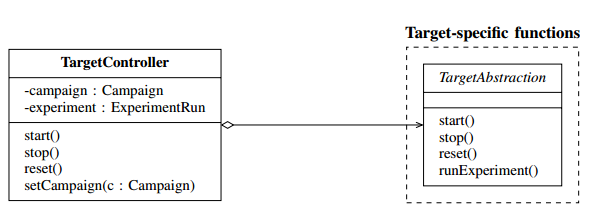
\includegraphics[width=400pt]{Pictures/Grinder_Extension}
	\caption{Abstract Target representation of GRINDER}
\end{center}
\end{figure}

\begin{figure}[H]
	\centering
	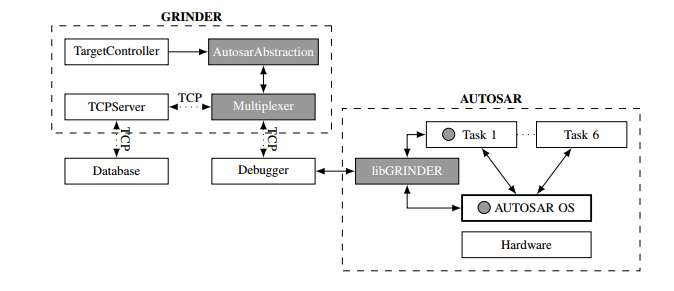
\includegraphics[width=400pt]{Pictures/GRINDER_Arch}
	\caption{GRINDER new arch.}\label{visina8}
\end{figure}
%------------------------------------------------

A case study is further done on Adaptive Cruise Control module. 
\begin{figure}[H]
	\centering
	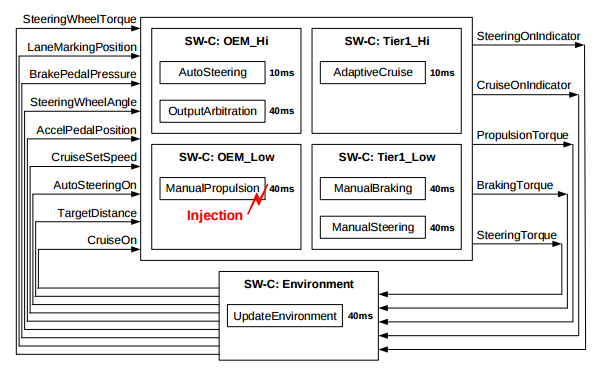
\includegraphics[width=400pt]{Pictures/ABS}
	\caption{ABS Module architecture}\label{abs}
\end{figure}


Four different scenarios tested:
\begin{itemize}
	\item Task timing error: Assess the correctness of the error detection and error mitigation of execution time monitoring. Analyze the propagation of the error with and without the presence of the timing errors.
	\item Interaction between the execution time monitoring and resource lock timing monitoring. Assess correctness and robustness of the mechanisms.
\end{itemize}

The task selection for monitoring ABS is shown below:
\begin{figure}[H]
	\centering
	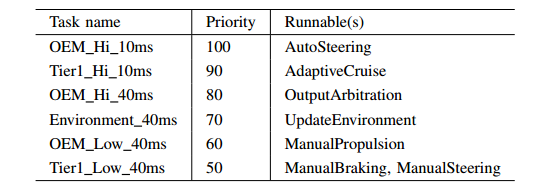
\includegraphics[width=400pt]{Pictures/Task}
	\caption{ACC task setup}\label{abs}
\end{figure}
\subsection{conclusion} % Sub-sub-section
Detailed description of scenarios, A good framework to test the mechanism of fault injection and different failure scenarios.
Can be used with possible change to JTAG interface to FTDI interface. Can be implemented as part of the eclipse plugin as as schedulability and testing mechanism.

\subsection{Links}
http://www1.deeds.informatik.tu-darmstadt.de/External/PublicationData/1/edcc-2015.pdf

